%%%%%%%%%%%%%%%%%%%%%%%%%%%%%%%%%%%%%%%%%%%%%%
%                insertmeeting
% 1) Title (something creative & funny?)
% 2) Date (MM/DD/YYYY)
% 3) Location (ex. Hagerty High School)
% 4) People/Committees Present 
% 5) Picture 
% 6) Start Time & Stop Time (ex. 12:30AM to 4:30PM)
%%%%%%%%%%%%%%%%%%%%%%%%%%%%%%%%%%%%%%%%%%%%%%
\insertmeeting 
	{Pushin PID} 
	{12/19/21} 
	{Hagerty High School}
	{Ritam}
	{Images/RobotPics/robot.jpg}
	{10:00 - 5:00}
	
\hhscommittee{Software}
\noindent\hfil\rule{\textwidth}{.4pt}\hfil
\subsubsection*{Goals}
\begin{itemize}
    \item Start editing roadrunner to our needs 

\end{itemize} 

\noindent\hfil\rule{\textwidth}{.4pt}\hfil

\subsubsection*{Accomplishments}
After a successful second meet, we realized that many other teams were starting to do the same tasks that we sought to complete in autonomous. This led to us thinking about how we could be different and work together with our alliance partner in autonomous, rather than us just sitting there or doing our normal autonomous routing of dropping the pre-loaded block, spinning the carousel and parking. We found that most of the time, the people who did the same tasks as us started on the side closest to the carousel as it was easier to do all of those tasks when close to the carousel. We found that if we started on the other side and picked up blocks, the 2 teams together could have a very high scoring autonomous, however our current way of writing our software with a basic PID controller would not suffice. This led us back to roadrunner, a motion planning library that allows for complex path following. This would be essential for us as we would need to perfectly be able to get through the gap autonomously and would allow us to be faster than just using the basic PID controller. We reverted back to when we had the roadrunner library in our directory and started to think about ways to change their programs up to work with our tricycle drive, however we first needed to figure out how everything worked. 



\hhscommittee{Hardware}
\noindent\hfil\rule{\textwidth}{.4pt}\hfil
\subsubsection*{Goals}
\begin{itemize}
    \item Learn how to make parts out of carbon fiber
	\item Create one of the carbon fiber sides with 3D printed molds

\end{itemize} 

\noindent\hfil\rule{\textwidth}{.4pt}\hfil

\subsubsection*{Accomplishments}
Although it has been a while since we designed the molds for our carbon fiber sides, our meet yesterday motivated us to start actually building one of the sides so that we can use them at a future competition. We are going to create the sides by layering carbon fiber cloth and epoxy over the mold, then we will place the mold and cloth inside a vacuum bag and use a vacuum pump to compress the layers of cloth onto the mold. 
To start the process, we got our 3d printed mold which we printed and put wax on a few days ago (Figure \ref{fig:121921_1}). The wax helps smooth out the bumps from the layers on the 3D printed part and will keep the carbon fiber from sticking to the sides, allowing us to remove the part from the mold when we are done. We then placed the mold onto a plate of glass and put tacky tape (which will be used to hold the vacuum bag down) around the mold (Figure \ref{fig:121921_2}). The next step was to cut sections of carbon fiber out of some plain weave carbon fiber cloth. We cut these sections to the right size so that they would fit exactly over the mold with as little extra material as possible (Figure \ref{fig:121921_3}). The carbon fiber cloth is weaved at 90 degree angles, which means that the plates will be easier to bend in the two directions where the fibers run. To remedy this issue, we cut some sections of the cloth at 45 degree angles and will overlap them with the other cloth so that the sides are strong in all directions. With 5 layers of cloth cut out, we mixed some epoxy and used paint brushes to apply it to the mold. We then put the first layer on the mold and painted more epoxy on top of that layer. We repeated this step for all of the layers, making sure to press the cloth into some of the tighter corners of the mold. On top of the carbon fiber, we added 2 layers that will help the process. The first layer, called peel-ply, is a thin cloth with small holes in it that will allow small amounts of epoxy to seep through. The top layer is a thicker layer of absorbent cloth which will suck up epoxy through the peel ply. These 2 layers will ensure that any excess epoxy is removed from the mold which will help reduce weight by leaving only enough epoxy to hold the carbon fiber together firmly. After adding all of these layers, we measured a sheet of plastic that we will use as the vacuum bag. We read that for the vacuum bag to properly compress the carbon fiber, that there should be 1.5 times the length needed to cover the part being compressed. This extra room prevents the bag from breaking when it is sucked down over the mold by the vacuum pump. The final step before we could start the pump was to attach the bag to the tacky tape that we put on the glass earlier. We also need to add pleats in the bag around parts of the mold that are raised up higher than the rest, which will give a more even distribution of force on the layers from the vacuum pump (Figure \ref{fig:121921_4}). 
Now it was time to turn on the vacuum pump and compress the layers. After turning on the pump, the bag was pulled tight over the part, pushing all of the layers down evenly onto the mold (Figure \ref{fig:121921_5}). Looking at the pressure indicator valve, we could see that our seal was only at 27.5 Hg or 13.5 psi a bit off from a perfect seal at 14.7 psi, so we looked around the edges of the bag, specifically around the pleats, pinching any cracks or bumps in the tacky tape shut. After going around and ensuring the seal was tight, we saw that the pressure was now about 29 Hg or about 14.25 psi which is much closer to the target of 14.7 psi. Feeling confident about our seal, we let the carbon fiber sit with the vacuum pump on for 6 hours. We are waiting excitedly to get the final piece out at the next meeting!

\begin{figure}[ht]
\centering
\begin{minipage}[b]{.48\textwidth}
  \centering
  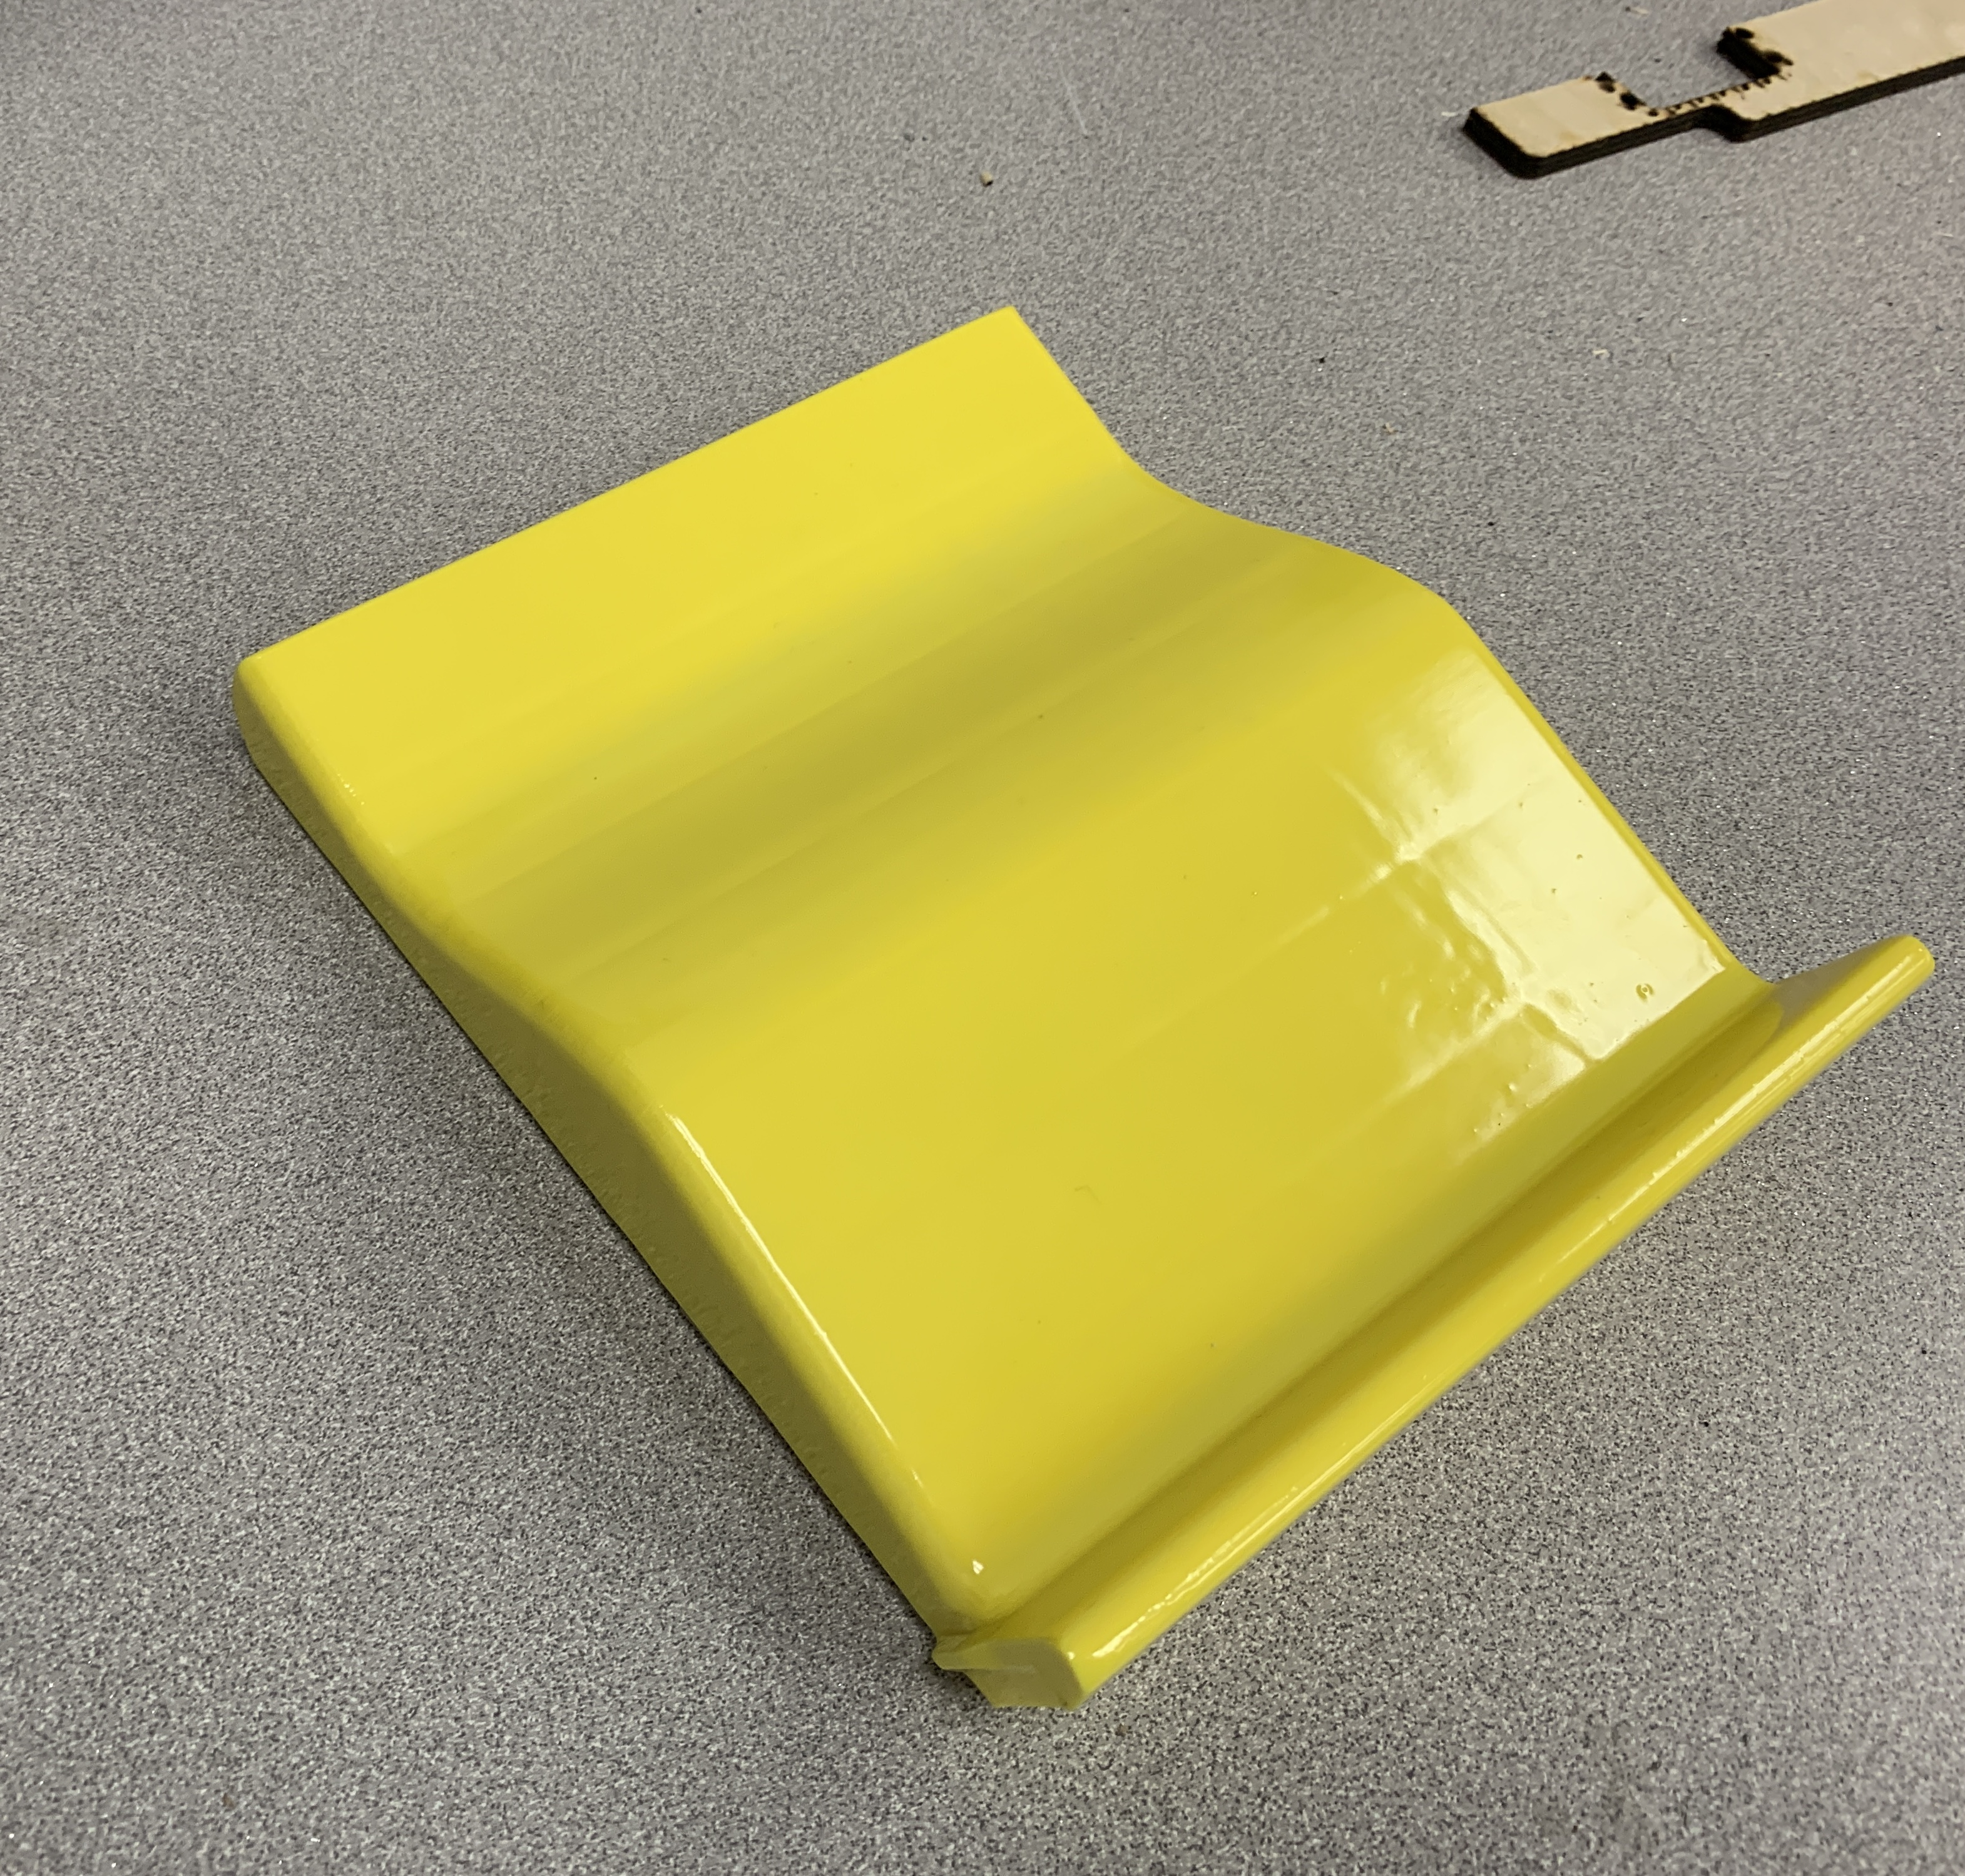
\includegraphics[width=0.95\textwidth]{Meetings/December/12-19-21/12-19-21_Hardware_Figure1 - Nathan Forrer.jpg}
  \caption{Our 3D printed}
  \label{fig:121921_1}
\end{minipage}%
\hfill%
\begin{minipage}[b]{.48\textwidth}
  \centering
  \includegraphics[width=0.95\textwidth]{Meetings/December/12-19-21/12-19-21_Hardware_Figure2 - Nathan Forrer.JPG}
  \caption{The mold structure}
  \label{fig:121921_2}
\end{minipage}
\end{figure}

\begin{figure}[ht]
\centering
\begin{minipage}[b]{.48\textwidth}
  \centering
  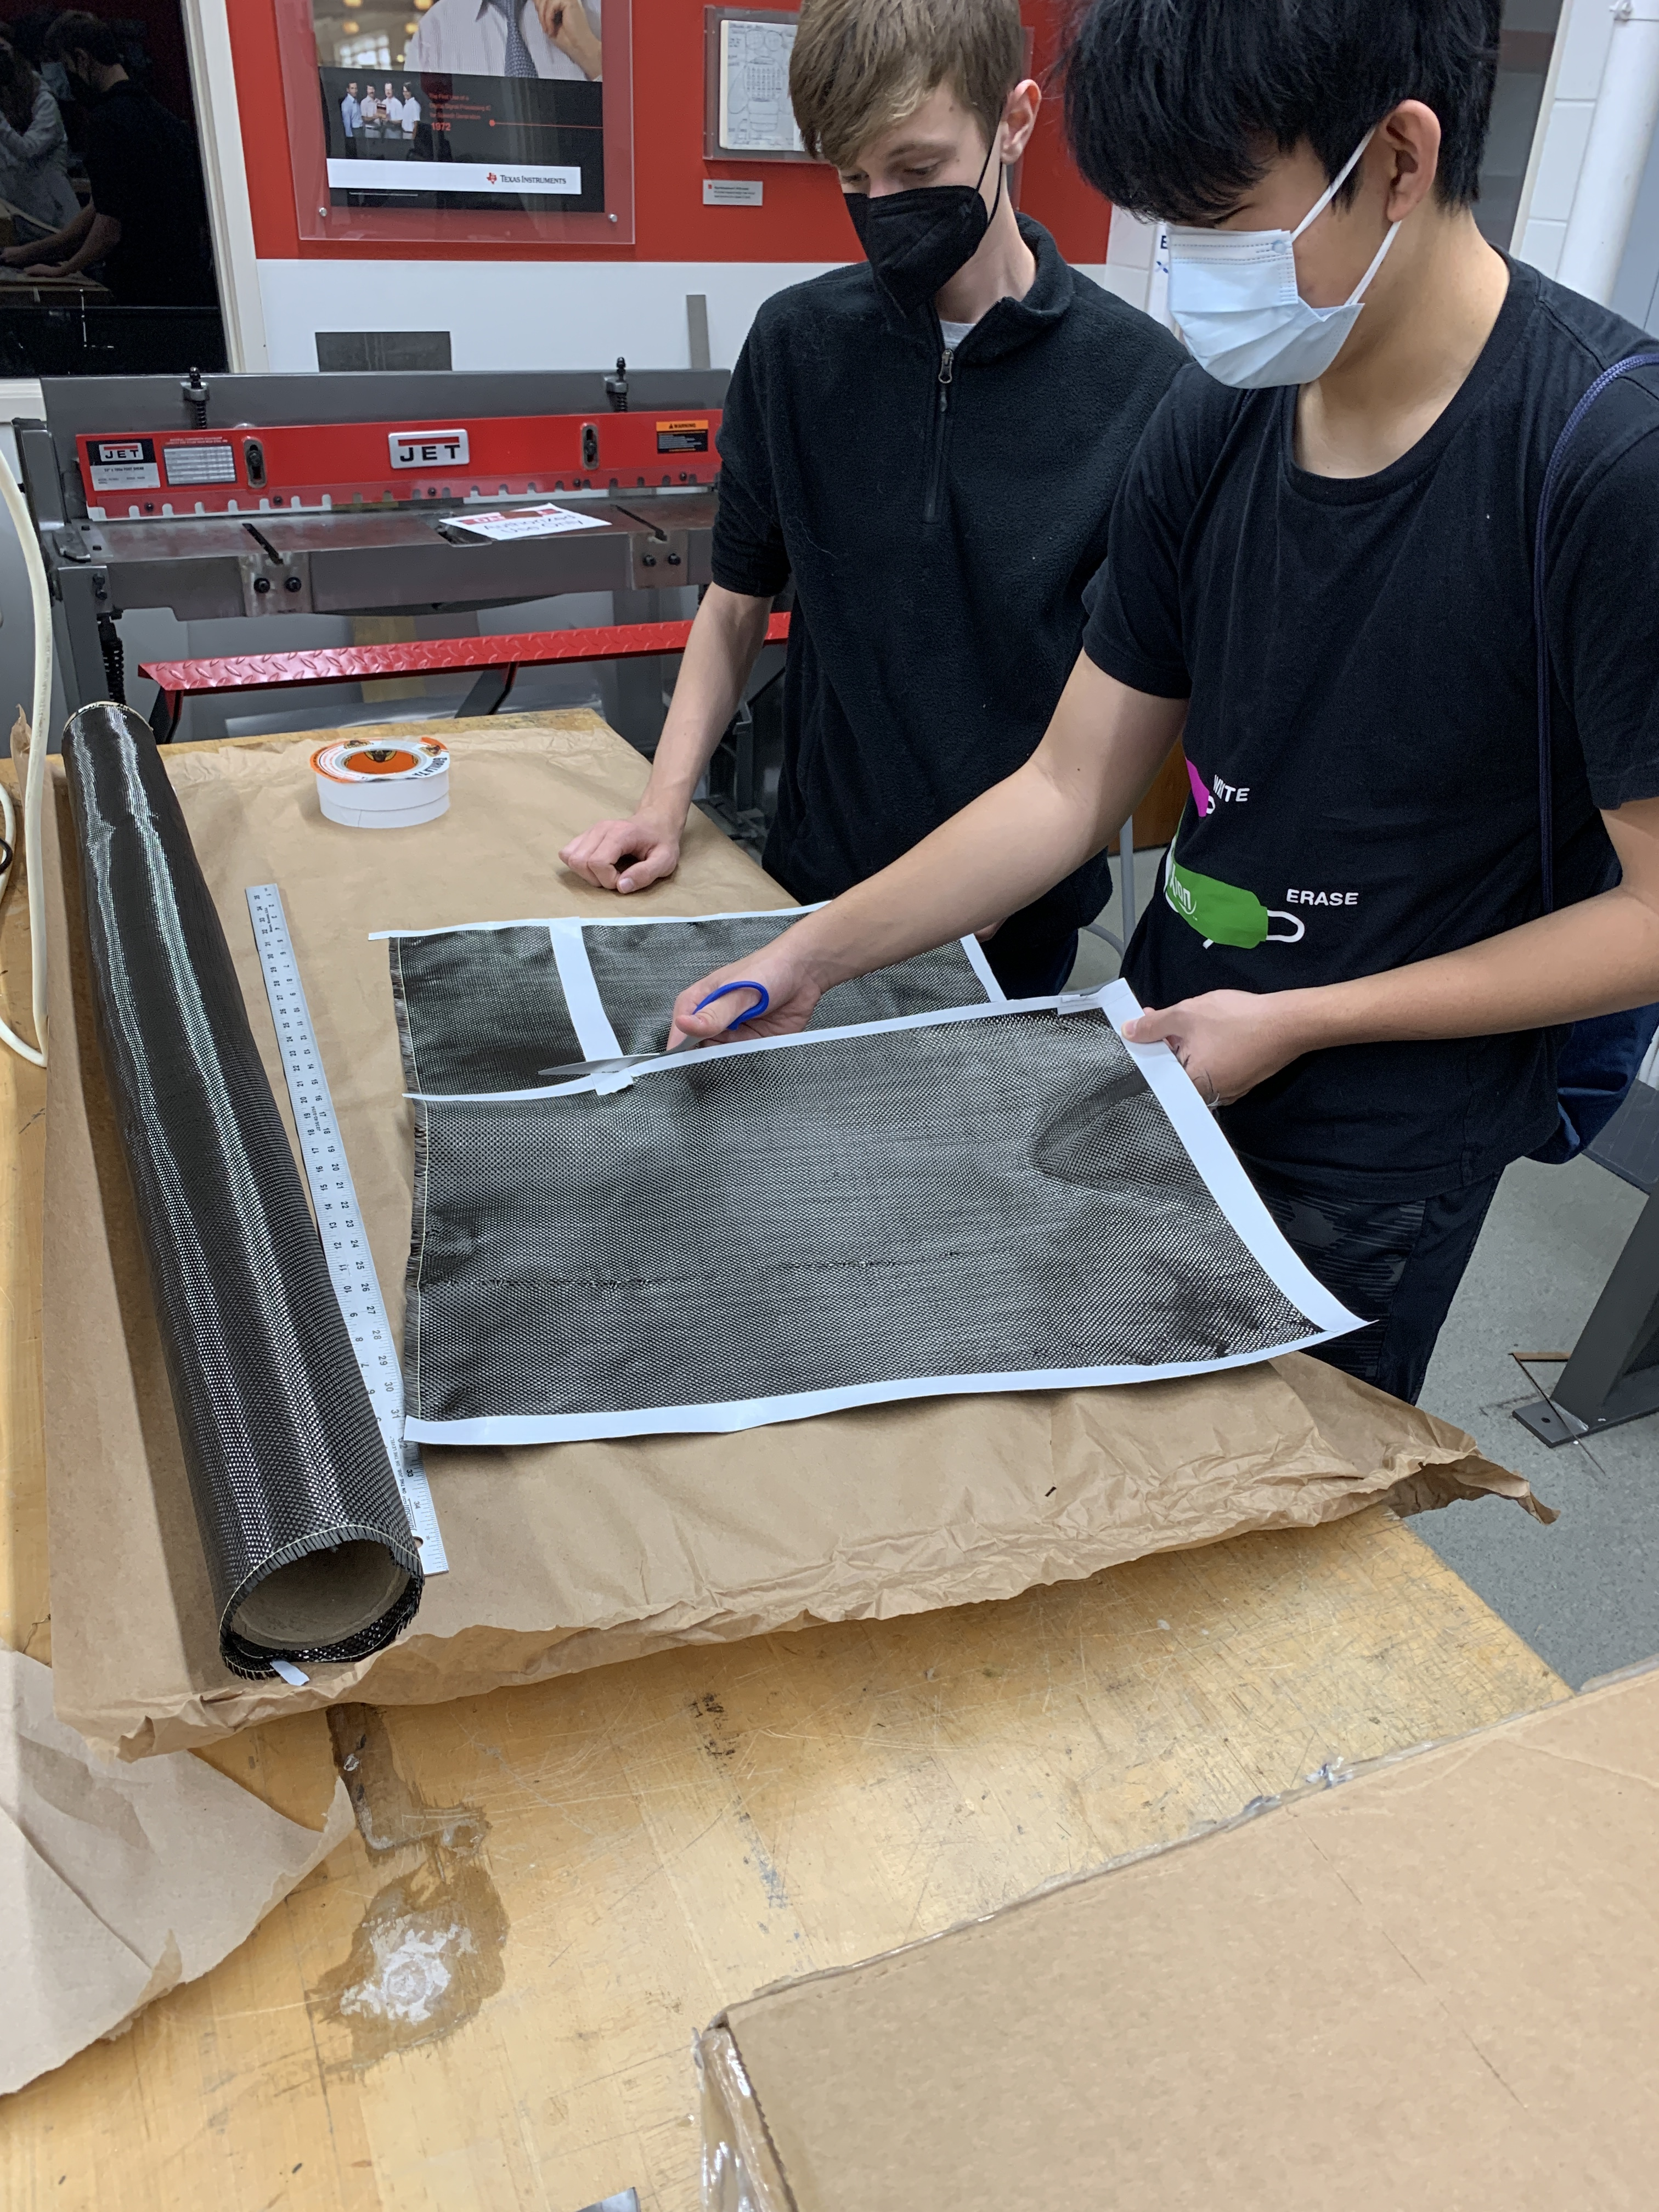
\includegraphics[width=0.95\textwidth]{Meetings/December/12-19-21/12-19-21_Hardware_Figure3 - Nathan Forrer.JPG}
  \caption{Cutting the plain weave}
  \label{fig:121921_3}
\end{minipage}%
\hfill%
\begin{minipage}[b]{.48\textwidth}
  \centering
  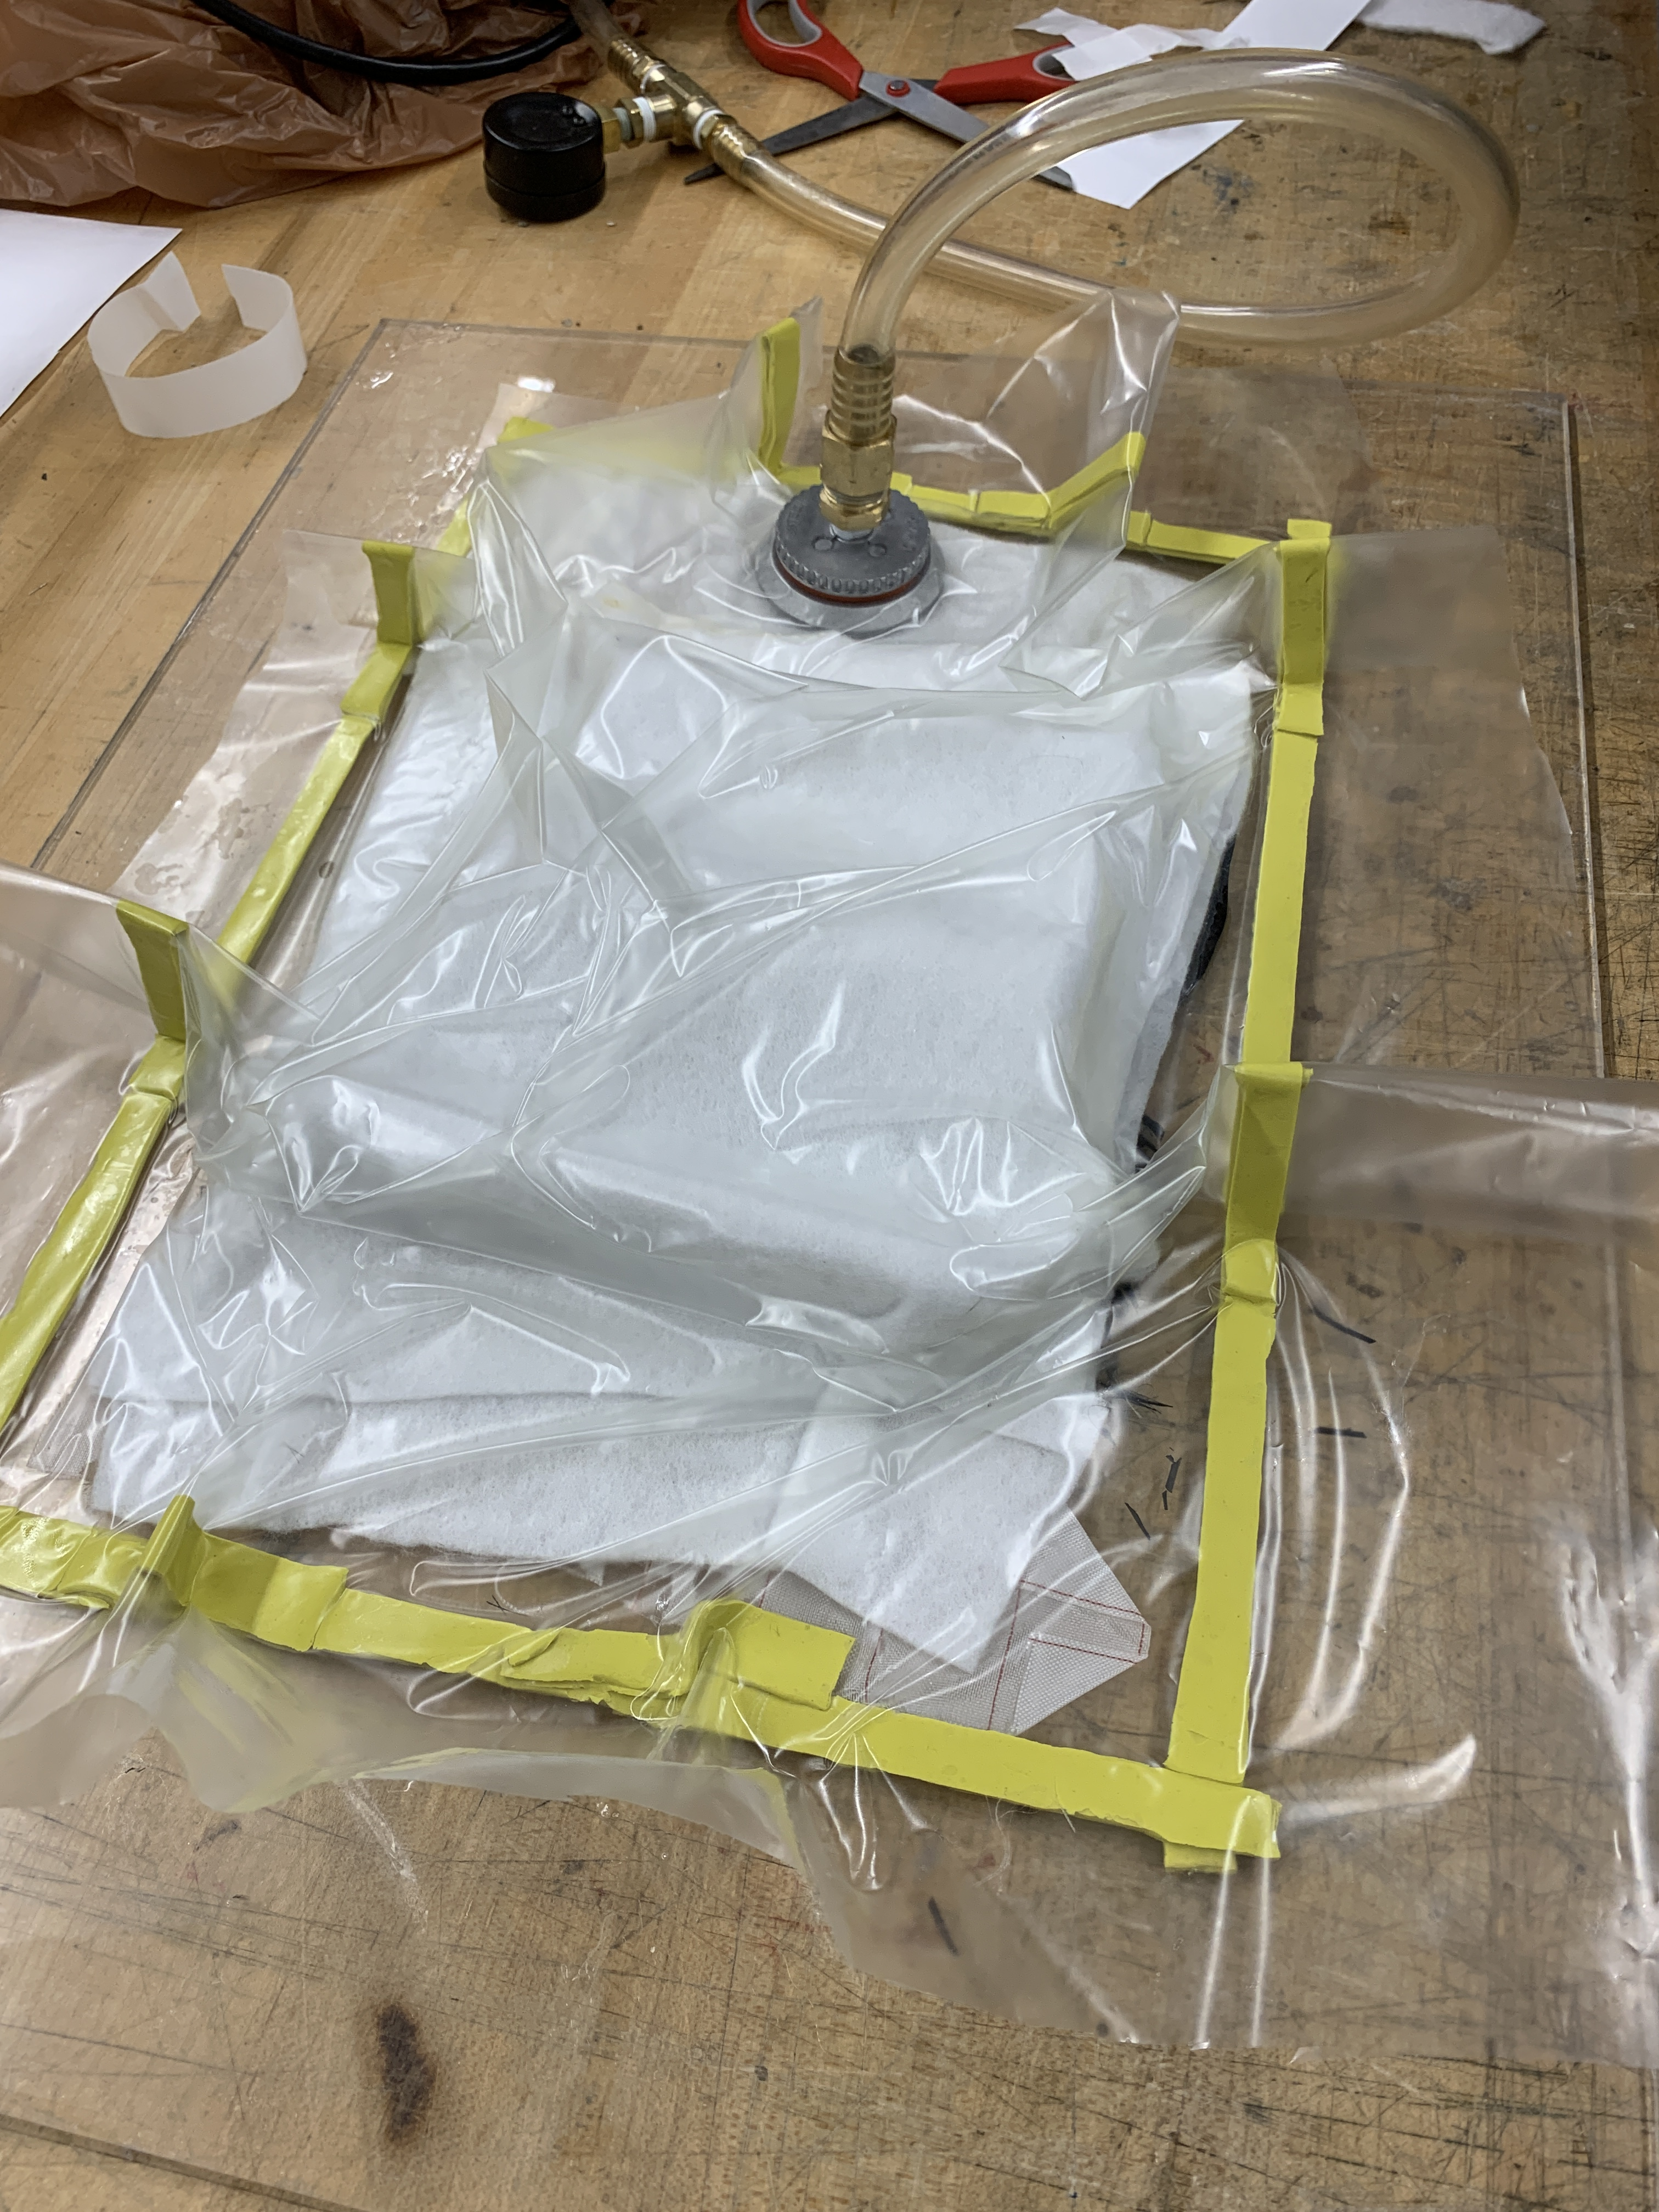
\includegraphics[width=0.95\textwidth]{Meetings/December/12-19-21/12-19-21_Hardware_Figure4 - Nathan Forrer.JPG}
  \caption{Using the vacuum pump}
  \label{fig:121921_4}
\end{minipage}
\end{figure}

\begin{figure}[htp]
\centering
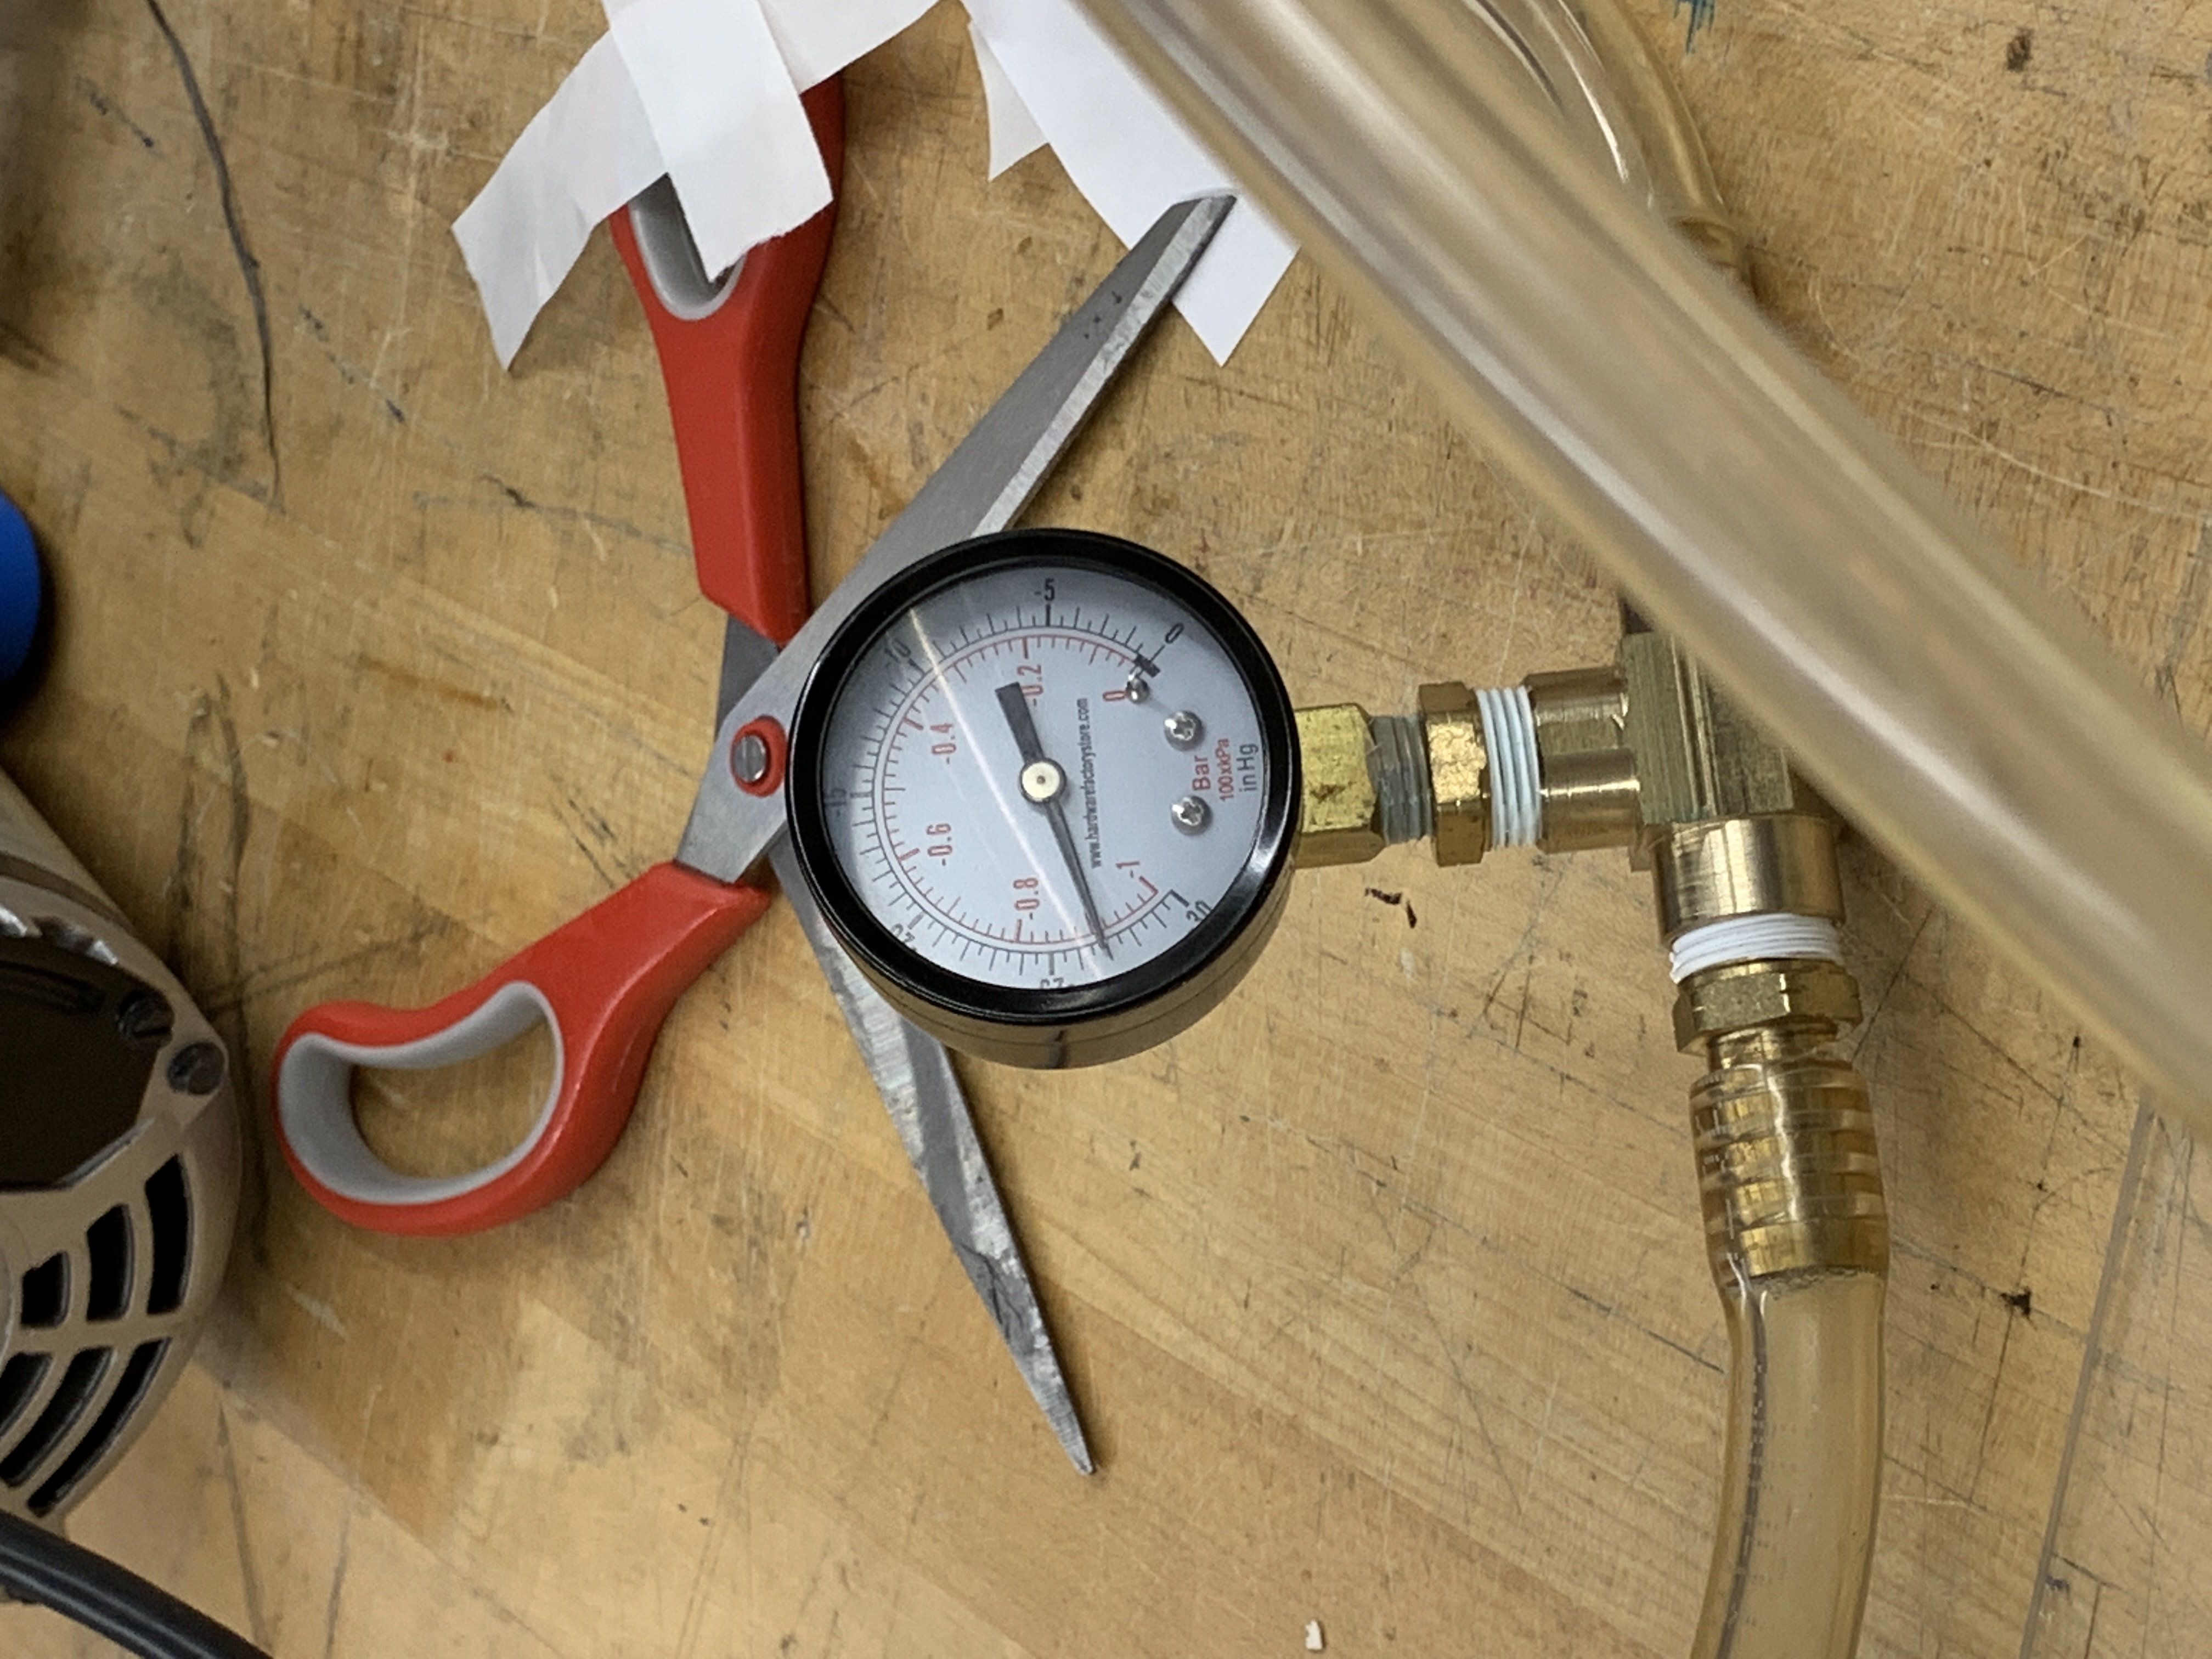
\includegraphics[width=0.95\textwidth, angle=0]{Meetings/December/12-19-21/12-19-21_Hardware_Figure5 - Nathan Forrer.JPG}
\caption{Pushing all the layers down}
\label{fig:121921_5}
\end{figure}
 

\whatsnext{
\begin{itemize}
    \item Figuring out how everything works together in roadrunner
    \item Get carbon fiber side out of vacuum bag
	  \item Asses effectivity of the process
	  \item Apply what we learned to the second carbon fiber side
\end{itemize} 
}

